%\documentclass[12pt]{report}
\documentclass[12pt,report,strict]{SANDreport/SANDreport}
\usepackage{pslatex}
\usepackage[FIGBOTCAP,normal,bf,tight]{subfigure}
\usepackage{draftwatermark}
\usepackage{ifthen}
\usepackage{nomenclature}
\usepackage{url}
\usepackage{enumitem}
\usepackage{multirow}
\usepackage{fancyvrb}
\usepackage{xcolor}
\usepackage{adjustbox}
\usepackage{changepage}
\usepackage{verbatim}
\usepackage{fancybox}
\usepackage[linkcolor=red]{hyperref}

%\def\SANDmain{}
%\def\SANDauthor{}
%\def\SANDnum{}
%\def\SANDprintDate{}

%\setlength{\parskip}{\baselineskip}%
%\setlength{\parindent}{0pt}%
\definecolor{shadecolor}{rgb}{.9, .9, .9}
\definecolor{yelgr}{RGB}{154, 205, 50}
\definecolor{lemon}{RGB}{255, 215, 0}
\definecolor{cmdcol}{RGB}{32, 178, 170}

\newenvironment{example}%
   {\par\noindent\adjustbox{margin=1ex,bgcolor=shadecolor,margin=0ex
       \medskipamount}\bgroup\minipage\textwidth\verbatim}%
   {\endverbatim\endminipage\egroup}
\newenvironment{inpusage}%
   {\par\noindent\adjustbox{margin=1ex,bgcolor=lemon,margin=0ex
       \medskipamount}\bgroup\minipage\textwidth\verbatim}%
   {\endverbatim\endminipage\egroup}
\newenvironment{interface}%
   {\par\noindent\adjustbox{margin=1ex,bgcolor=lemon,margin=0ex
       \medskipamount}\bgroup\minipage\textwidth}%
   {\endminipage\egroup}
\newcommand{\param}[2]{\noindent\texttt{#1}%
  \begin{adjustwidth}{2.5em}{0pt}#2\end{adjustwidth}}
\newcommand{\usage}[1]{\indent\hspace{2.5em}\texttt{#1}}

\newcommand{\vnv}{V\&V}
\newcommand{\payette}{\texttt{payette}}
\newcommand{\med}{\texttt{MED}}
\newcommand{\pmd}{\texttt{MMD}}
\newcommand{\mml}{\texttt{matmodlab}}
\newcommand{\mmd}{\texttt{mmd}}
\newcommand{\mmv}{\texttt{mmv}}
\newcommand{\bldm}{\texttt{buildmtls}}
\newcommand{\runtests}{\texttt{runtests}}
\newcommand{\exodusii}{{\sc\texttt{ExodusII}}}
\newcommand{\fpy}[1]{\texttt{f2py}}
\newcommand{\paraview}[1]{{\sc\texttt{paraview}}}
\newcommand{\pprepro}[1]{{\texttt{pprepro}}}
\newcommand{\us}{\underline{  }}
\newcommand{\uus}{\us\us{}}
\newcommand{\sol}{\texttt{solid}}
\newcommand{\eos}{\texttt{eos}}
\newcommand{\wf}{\Tensor{w}{}{}}
\newcommand{\vc}{\text{v}}
\newcommand{\PrescStress}{\Tensor{\sigma}{}{p}}

% --- xml
\renewcommand{\tag}[1]{\texttt{<#1>}}
\newcommand{\reqdtag}[1]{\Red{\texttt{<#1>}}}
\newcommand{\gat}[1]{\texttt{<\textbackslash{}#1>}}
\newcommand{\supporting}[1]{\texttt{Supporting Drivers: #1}}
\newcommand{\element}[4][0in]{%
  \indent\hspace{#1}\tag{#2 #3}\\%
  \indent\hspace{.2in}#4\\%
  \indent\hspace{#1}\gat{#2}}
\newcommand{\attr}[2][]{\ifthenelse{\equal{#1}{}}{\texttt{#2}}{\texttt{#2="#1"}}}


% ---------------------------------------------------------------------------- %
\title{\mml{} \\ a Material Model Laboratory}
\author{Tim Fuller \\
  Computational Structural Mechanics and Applications \\
  Sandia National Laboratories\\
  P.O. Box 5800\\
  Albuquerque, NM 87185-9999 \\
  tjfulle@sandia.gov }
\date{}


% ---------------------------------------------------------------------------- %
\SANDnum{SAND2002-xxxx}
\SANDprintDate{October 2013}
\SANDauthor{Tim Fuller}

\begin{document}
\maketitle

\begin{abstract}
  The Material Model Laboratory (\mml{}) is a suite of tools whose purpose is
  to aid in the rapid development and testing of material models. \mml{} is
  made up of several components, the most notable being the Material Model
  Driver \mmd{}. \mmd{} can be thought to drive a single material point of a
  finite element simulation through very specific user designed paths. This
  permits exercising material models in ways not possible in finite element
  calculations, desgining verification and validation tests of the material
  response, among others. \mml{} is a small suite of tools at the developers
  disposal to aid in the design and implementation of material models in
  larger finite element host codes. It is also a useful tool to analysists for
  understanding and parameterizing a material's response to deformation.
\end{abstract}

\cleardoublepage		% TOC needs to start on an odd page
\tableofcontents
\listoffigures
\listoftables

\SANDmain		% Start the main part of the report

% ----------------------------------------------------------------------------- %
\chapter{Introduction to \mml{}}
\label{chap:intro}
The Material Model Laboratory (\mml{}) is a suite of tools whose purpose is to
aid in the rapid development and testing of material models. \mml{} is made up
of several components, the most notable being the Material Model Driver
\mmd{}. \mmd{} can be thought to drive a single material point of a finite
element simulation through very specific user designed paths. This permits
exercising material models in ways not possible in finite element
calculations, desgining verification and validation tests of the material
response, among others. \mml{} is a small suite of tools at the developers
disposal to aid in the design and implementation of material models in larger
finite element host codes. It is also a useful tool to analysists for
understanding and parameterizing a material's response to deformation.

The core of \mml{} code base is written in Python and leverages Python's
object oriented programming (OOP) design. OOP techniques are used throughout
\mml{} to setup and manage simulation data. Computationally heavy portions of
the code, and the material models themselves are written in Fortran for its
speed and ubiquity in scientific computing. Calling Fortran procedures from
Python is made possible by the \fpy{} module, standard in Numpy, that compiles
and creates Python shared object libraries from Fortran sources.

Output files from \mml{} simulations are in the \exodusii{} \cite{exodus}
database format, devloped at Sandia National Labs for storing finite element
simulation data. Since \mml{} is designed to be used by material model
developers, it is expected that the typical user will want access to
\emph{all} available output from a material model, thus all simulation
data is written to the output database. \exodusii{} database files can be
visualized via the \mmv{} utility, in addition to other visualization packages
such as \paraview{} \cite{paraview}.

\mml{} is free software released under the MIT License.

% ----------------------------------------------------------------------------- %
\section{Why a Single Element Driver?}
\label{sec:why}
Due to their complexity, it is often over kill to use a finite element code
for constitutive model development. In addition, features such as artificial
viscosity can mask the actual material response from constitutive model
development. Single element drivers allow the constituive model developer to
concentrate on model development and not the finite element response. Other
advantages of \mml{} (or, more generally, of any stand-alone
constitutive model driver) are

\begin{itemize}
  \item \mml{} is a very small, special purpose, code. Thus, maintaining and
  adding new features to \mml{} is very easy.

  \item Simulations are not affected by irrelevant artifacts such as
  artificial viscosity or uncertainty in the handling of boundary conditions.

  \item It is straightforward to produce supplemental output for deep analysis
  of the results that would otherwise constitute an unnecessary overhead in a
  finite element code.

  \item Specific material benchmarks may be developed and automatically run
  quickly any time the model is changed.

  \item Specific features of a material model may be exercised easily by the
  model developer by prescribing strains, strain rates, stresses, stress
  rates, and deformation gradients as functions of time.
\end{itemize}

% ----------------------------------------------------------------------------- %
\section{Why Python?}
\label{sec:why-python}
Python is an interpreted, high level object oriented language. It allows for
writing programs rapidly and, because it is an interpreted language, does not
require a compiling step. While this might make programs written in python
slower than those written in a compiled language, modern packages and
computers make the speed up difference between python and a compiled language
for single element problems almost insignificant.

For numeric computations, the NumPy and SciPy modules allow programs written
in Python to leverage a large set of numerical routines provided by LAPACK,
BLASPACK, EIGPACK, etc. Python's APIs also allow for calling subroutines
written in C or Fortran (in addition to a number of other languages), a
prerequisite for model development as most legacy material models are written
in Fortran. In fact, most modern material models are still written in Fortran
to this day.

Python's object oriented nature allows for rapid installation of new material
models.

% ----------------------------------------------------------------------------- %
\section{Historical Background}
\label{sec:background}
When I was a graduate student at the University of Utah I had the good fortune
to have as my advisor Dr.~Rebecca Brannon. Prof.~Brannon instilled in me the
necessity to develop material models in small special purpose drivers, free
from the complexities of larger finite element codes. To this end, I began
developing material models in Prof.~Brannon's \med{} driver (available upon
request from Prof.~Brannon). The \med{} driver was a special purpose driver
for driving material models through predefined strain paths. After completing
graduate school I began employment as a member of the Technical Staff at
Sandia National Labs. Among the many projects I worked on was the development
of material models for geologic applications. There, I found need to drive the
material models through prescribed stress paths to match experimental records.
This capability was not present in the \med{} and I sought a different
solution. The solution came from the \pmd{} driver, created years earlier at
Sandia, by Tom Pucick. The \pmd{} driver had the capability to drive material
models through prescribed stress and strain paths, but also lacked many of the
IO features of the \med{}. And so, for some time I used both the \med{} and
\pmd{} drivers in applications that suited their respective strengths. After
some time using both drivers, I decided to combine the best features of each
in to my own driver. Both the \med{} and \pmd{} drivers were written in
Fortran and I decided to write the new driver in Python so that I could
leverage the large number of builtin libraries. The Numpy and Scipy Python
libraries would be used for handling most number crunching. The new driver
came to be known as \payette{}. \payette{} added many unique capabilities and
became a capable piece of software used by other staff members at Sandia. But,
\payette{} suffered from the fact that it was my first foray in to programming
with Python. After some time, the bloat and bad programming practices with
\payette{} caused me to spend a few weekends re-writing it in to what is now
known as \mml{}.

% ----------------------------------------------------------------------------- %
\section{Obtaining \mml{}}
\label{sec:obtain}
\mml{} is an open source project licensed under the MIT license. A copy of may
be obtained from \url{https://github.com/tjfulle/matmodlab}

% ----------------------------------------------------------------------------- %
\section{About This Guide}
\label{sec:about}
\mml{} is developed as a tool for developers and analysts who care to
understand the responses of material models to specific deformation paths. The
target audience is assumed to have a basic knowledge of continuum mechanics
and familiarity with other finite element codes.  Accordingly, concepts of
continuum mechanics and finite element methods are not described in detail and
programing techniques are also not described.

% ----------------------------------------------------------------------------- %
\chapter{\mml{} Quick Start Guide}
\label{chap:quick}
This guide provides an outline for building and running \mml{}.

\textbf{Build \mml{}} See Chapter \ref{chap:build}.
\begin{itemize}
  \item Download \mml{} and setup environment
  \item \$ \verb|cd $MMLROOT/toolset && ./setup.py|
  \item \$ \bldm{}
\end{itemize}

\textbf{Prepare Input} Inputs are xml specification files. See Chapters
\ref{chap:inpov} - \ref{chap:inpopt}.
\begin{itemize}
  \item Set up the desired simulation path.
  \item Add material model.
  \item Add desired extraction requests.
\end{itemize}

\textbf{Run}
\begin{itemize}
  \item \$ \mmd{} [options] \emph{runid} [,\emph{runid\_1}, $\ldots$,
  \emph{runid\_n}]\\
  \emph{runid} is prefix of ``.xml'' file.
  \item Complete list of options given by \\ \$ \texttt{mmd -h}
\end{itemize}

\textbf{Postprocess}
\begin{itemize}
  \item \$ \mmv{} \emph{runid} [,\emph{runid\_1}, $\ldots$,
  \emph{runid\_n}]
  \item \paraview{} also reads exodus files.
\end{itemize}


% ----------------------------------------------------------------------------- %
\chapter{Building \mml{}}
\label{chap:build}
\mml{}'s code base is largely written in Python and requires no additional
compiling. However, several fortran procedures, the \exodusii{} third party
library, and material models written in fortran must be built.

% ----------------------------------------------------------------------------- %
\section{System and Software Requirements}
\label{sec:sys}
\mml{} has been built and tested extensively on several versions of linux and
the Apple Mac OSX operating systems. It is unknown whether or not \mml{}
will run on Windows.

\mml{} requires the following software installed for your platform:

\begin{itemize}
  \item Python 2.7
  \item NumPy 1.6
  \item SciPy 0.10
  \item A fortran compiler
\end{itemize}

The required software may be obtained in several ways, though all development
has been made using Enthought Canopy (\url{http://http://www.enthought.com}).

A note on the fortran compiler.  It is recommended to use the same fortran
compiler to build \mml{} components that was used to build SciPy.

% ----------------------------------------------------------------------------- %
\section{Installation}
\label{sec:install}
Ensure that all \mml{} prerequisites are installed and working properly before
proceeding.

% ----------------------------------------------------------------------------- %
\subsection{Set Environment and Path}
\label{sec:setup}

\begin{description}[leftmargin=!,labelwidth=\widthof{\texttt{MMLMTLS}}]
  \item[\texttt{MMLROOT}] Optional, name of installation directory
  \item[\texttt{PATH}] \verb|$MMLROOT/toolset:$PATH|
  \item[\texttt{MMLMTLS}] ``:'' separated list of paths to directories
  containing user defined material models. See Section \ref{sec:usrbld}.
\end{description}

% ----------------------------------------------------------------------------- %
\subsection{Set Up}
\label{sec:setup-1}
Set up and build the TPLs.
%
\begin{verbatim}
$ cd $MMLROOT/toolset
$ python setup.py
\end{verbatim}
%
In addition to building the TPLs, \texttt{setup.py} generates the following
executable scripts
%
\begin{description}[leftmargin=!,labelwidth=\widthof{\texttt{buildmtls}}]
  \item[\texttt{buildmtls}] Build material models
  \item[\texttt{mml}] Run \mml{} simulations
  \item[\texttt{exdump}] Read a \mml{} output and dumps requested variables
  to ascii columnar files
  \item[\texttt{mmv}] 2D plots of \mml{} output
  \item[\texttt{runtests}] Run the regression tests
\end{description}
%
Each script is a wrapper to another \mml{} Python file. In the wrapper,
relevant environment variables are set (e.g., \verb|$PYTHONPATH|) and the
correct Python executable (the one used to set up) is used to interpret the
\mml{} source file.  The full set of options for each script is obtained by
%
\begin{verbatim}
$ scriptname -h
\end{verbatim}
%
where \texttt{scriptname} is the name of the script.

The TPLs will build the first time \mml{} is setup.
Thereafter after, only the executable scripts are rewritten.  Execute

\begin{verbatim}
$ python setup.py -h
\end{verbatim}
for options to rebuild the TPLs.

% ----------------------------------------------------------------------------- %
\subsection{Build}
\label{sec:bld}
Build the material libraries
\begin{verbatim}
$ buildmtls
\end{verbatim}

% ----------------------------------------------------------------------------- %
\subsection{Test the Installation}
\label{sec:test-install}
To test \mml{} after installation, execute

\begin{verbatim}
$ runtests [-j N]
\end{verbatim}
%
which will run \mml{} regression tests.

% ----------------------------------------------------------------------------- %
\subsection{Troubleshooting}
\label{sec:trouble}
If you experience problems when building/installing/testing \mml{}, you can
ask help from \mml{} developers. Please include the following information
in your message:

\begin{itemize}
  \item Platform information OS, its distribution name and version information
  etc.
\begin{verbatim}
$ python -c "import os,sys;print os.name,sys.platform"
$ uname -a
\end{verbatim}

  \item Information about C,C++,Fortran compilers/linkers as reported by the
  compilers when requesting their version information, e.g., the output of
\begin{verbatim}
$ gcc -v
$ gfortran --version
\end{verbatim}

  \item Python version
\begin{verbatim}
$ python -c "import sys;print sys.version"
\end{verbatim}

\item NumPy version
\begin{verbatim}
$ python -c "import numpy;print numpy.__version__"
\end{verbatim}

\item SciPy version
\begin{verbatim}
$ python -c "import scipy;print scipy.__version__"
\end{verbatim}

\item Feel free to add any other relevant information.
\end{itemize}

% ----------------------------------------------------------------------------- %
\chapter{\mml{} Solution Method}
\label{chap:solmeth}
\mml{} exercises a material model directly by ``driving'' it through user
specified paths using a designated driver. Currently installed drivers are the
\sol{} and \eos{} drivers. For each driver type, \mml{} computes an increment
in deformation for a given step and requires that the material model update
the stress in the material to the end of that step, given the current state
and an increment in deformation. Because of the similarity of the material
model interface in \mml{} with many commercial finite element codes,
transitioning material models developed and tested in \mml{} to full finite
element codes should be an easy process. In this chapter, the role and
importance of the material model in a finite element procedure is reviewed.
The solution method adopted by each driver in \mml{} is then described and
compared with that of finite elements.

% ----------------------------------------------------------------------------- %
\section{The Role of the Material Model in Continuum Mechanics}
\label{sec:roleofmatmod}

% ----------------------------------------------------------------------------- %
\subsection{Conservation Laws}
\label{sec:cons-laws}
Conservation of mass, momentum, and energy are the central tenets of the
analysis of the response of a continuous media to deformation and/or load.
Each conservation law can be summarized by the following statement

\begin{minipage}{\textwidth}
\begin{center}
  \fbox{\begin{Bcenter}Time rate of\\ change of\\ quantity\end{Bcenter}} =
  \fbox{\begin{Bcenter}Rate of\\ production\\ in the\\ interior\end{Bcenter}} +
  \fbox{\begin{Bcenter}Flux\\ through the\\ boundary\end{Bcenter}}
\end{center}
\end{minipage}

Mathematically, the conservation laws for a point in the continuum are
%
\begin{itemize}
  \item Conservation of mass
  \begin{displaymath}
    \dDensity + \Density\Del\DotProd\dDisplacement = 0
  \end{displaymath}

  \item Conservtion of momentum per unit volume
  \begin{displaymath}
    \Density\Der{}{t}\dDisplacement =
    \underset{\text{internal forces}}{\boxed{\Del\DotProd\Stress}} +
    \underset{\text{body forces}}{\boxed{\BodyForce}}
  \end{displaymath}

  \item Conservation of energy per unit volume
  \begin{displaymath}
    \Density\Der{}{t}\Energy =
    \underset{\text{heat source}}{\boxed{\Density s}} +
    \underset{\text{strain energy}}{\boxed{\Stress\DDotProd\dStrain}} +
    \underset{\text{heat flux}}{\boxed{\Del\DotProd\HeatFlux}}
  \end{displaymath}
\end{itemize}
%
where $\Displacement$ is the displacement, $\Density$ the mass density,
$\Stress$ the stress, $\dStrain$ the rate of strain, $\BodyForce$ the body
force per unit volume, $\HeatFlux$ the heat flux, $s$ the heat source, and
$\Energy$ is the internal energy per unit mass.

In solid mechanics, mass is conserved trivially, and many problems are
adiabatic or isotrhermal, so that only the momentum balance is explicitly
solved
\begin{equation}
  \label{eq:mbal}
  \Density\Der{}{t}\dDisplacement =
  \underset{\text{internal forces}}{\boxed{\Del\DotProd\Stress}} +
  \underset{\text{body forces}}{\boxed{\BodyForce}}
\end{equation}

The balance of linear momentum is the continuum mechanics generalization of
Newton's second law $F=ma$.

The first term on the RHS of \eqref{eq:mbal} represents the internal
forces, which arise in the medium to resist imposed deformation. This
resistance is a fundamental response of matter and is given by the divergence
of the stress field.

The balance of linear momentum represents an initial boundary value problem
for applications of interest in solid dynamics:

\begin{equation}
  \label{eq:ibvp}
  \begin{aligned}
    \Density\Der{}{t}\dDisplacement = \Del\DotProd\Stress + \BodyForce&
    &&\quad\text{in }\Omega \\
    \Displacement = \Displacement_0& &&\quad\text{on }\Gamma_0 \\
    \Stress\DotProd\normal = \Traction& &&\quad\text{on }\Gamma_t \\
    \dDisplacement\left(\position, 0\right) =
    \dDisplacement_0\left(\position\right)&
    &&\quad\text{on }\position\in\Omega
  \end{aligned}
\end{equation}

\subsection{The Finite Element Method}
\label{sec:femeth}
The form of the momentum equation in \eqref{eq:ibvp} is termed the
\textbf{strong} form. The strong form of the initial BVP problem can also be
expressed in the weak form by introducing a test function $\wf$ and
integrating over space
\begin{equation}
  \label{eq:ibvp-1}
  \begin{aligned}
    \int_{\Omega}\wf\DotProd\left(
      \Del\DotProd\Stress + \BodyForce - \Density\Der{}{t}\dDisplacement
    \right)\,d\Omega& &&\quad \forall \wf \\
    \Displacement = \Displacement_0& &&\quad\text{on }\Gamma_0 \\
    \Stress\DotProd\normal = \Traction& &&\quad\text{on }\Gamma_t \\
    \dDisplacement\left(\position, 0\right) =
    \dDisplacement_0\left(\position\right)&
    &&\quad\text{on }\position\in\Omega
  \end{aligned}
\end{equation}

Integrating \eqref{eq:ibvp-1} by parts allows the traction boundary conditions
to be incorporated in to the governing equations
\begin{equation}
  \label{eq:weak}
  \begin{aligned}
    \int_{\Omega}\Density\wf\DotProd\Acceleration +
    \Stress\DDotProd\Del\wf\,d\Omega
    = \int_{\Omega}\wf\DotProd\BodyForce\,d\Omega +
    \int_{\Gamma}\wf\DotProd\Traction\,d\Gamma_{t}& &&\forall \wf \\
    %
    \Displacement = \Displacement_0& &&\quad\text{on }\Gamma_0 \\
    \dDisplacement\left(\position, 0\right) =
    \dDisplacement_0\left(\position\right)&
    &&\quad\text{on }\position\in\Omega
  \end{aligned}
\end{equation}

This form of the IBVP is called the \textbf{weak} form.  The weak form
poses the IBVP as a integro-differential equation and eliminates singularities
that may arise in the strong form.  Traction boundary conditions are
incorporated in the governing equations.  The weak form forms the basis for
finite element methods.

In the finite element method, forms of $\wf$ are assumed in subdomains
(elements) in $\Omega$ and displacements are sought such that the force
imbalance $R$ is minimized:

\begin{equation}
  \label{eq:resid}
  R = \int_{\Omega}\wf\DotProd\BodyForce\,d\Omega +
  \int_{\Gamma}\wf\DotProd\Traction\,d\Gamma_{t} -
 \int_{\Omega}\Density\wf\DotProd\Acceleration + \Stress\DDotProd\Del\wf\,d\Omega
\end{equation}

The equations of motion as described in \eqref{eq:resid} are not closed, but
require relationships relating $\Stress$ to $\Displacement$

\begin{center}
  \fbox{Constitutive model $\longrightarrow$ relationship between $\Stress$
    and $\Displacement$}
\end{center}

In the typical finite element procedure, the host finite element code passes
to the constitutive routine the stress and material state at the beginning of
a finite step (in time) and kinematic quantities at the end of the step. The
constitutive routine is responsible for updating the stress to the end of the
step. At the completion of the step, the host code then uses the updated
stress to compute kinematic quantities at the end of the next step. This
process is continued until the simulation is completed. The host finite
element handles the allocation and management of all memory, including memory
required for material variables.

% ----------------------------------------------------------------------------- %
\section{Solution Procedure}
\label{sec:mmlsol}
In addition to providing a platform for material model developers to formulate
and test constitutive routines, \mml{} aims to provide users of material
models an independent platform to exercise, parameterize, and compare material
responses against single element finite element simulations. To this end, the
solution procedure in \mml{} is similar to that of the finite element method,
in that the host code (\mml{}) provides to the constitutive routine a measure
of deformation at the end of a finite step and expects the updated stress in
return. However, rather than solve the momentum equation at the beginning of
each step and advancing kinematic quantities to the step's end, \mml{}
retrieves updated kinematic quantities from user defined tables and/or
functions.

The path through which a material is exercised is defined by piecewise
continuous ``legs'' in which components of the ``control type'' $c_{i}$ are
specified at discrete points in time, shown in Figure \ref{fig:path}.  The
$c_{i}$ are used to obtain a sequence of piecewise constant strain rates that
are used to advance the kinematic state.  Supported control types are strain,
strain rate, stress, stress rate, deformation gradient, displacement, and
velocity.  ``Mixed-modes'' of strain and stress (and their rates) are
supported.  Components of displacement and velocity control are applied only
to the ``+'' faces of a unit cube centered at the coordinate origin.

\begin{figure}[ht]
  \centering
  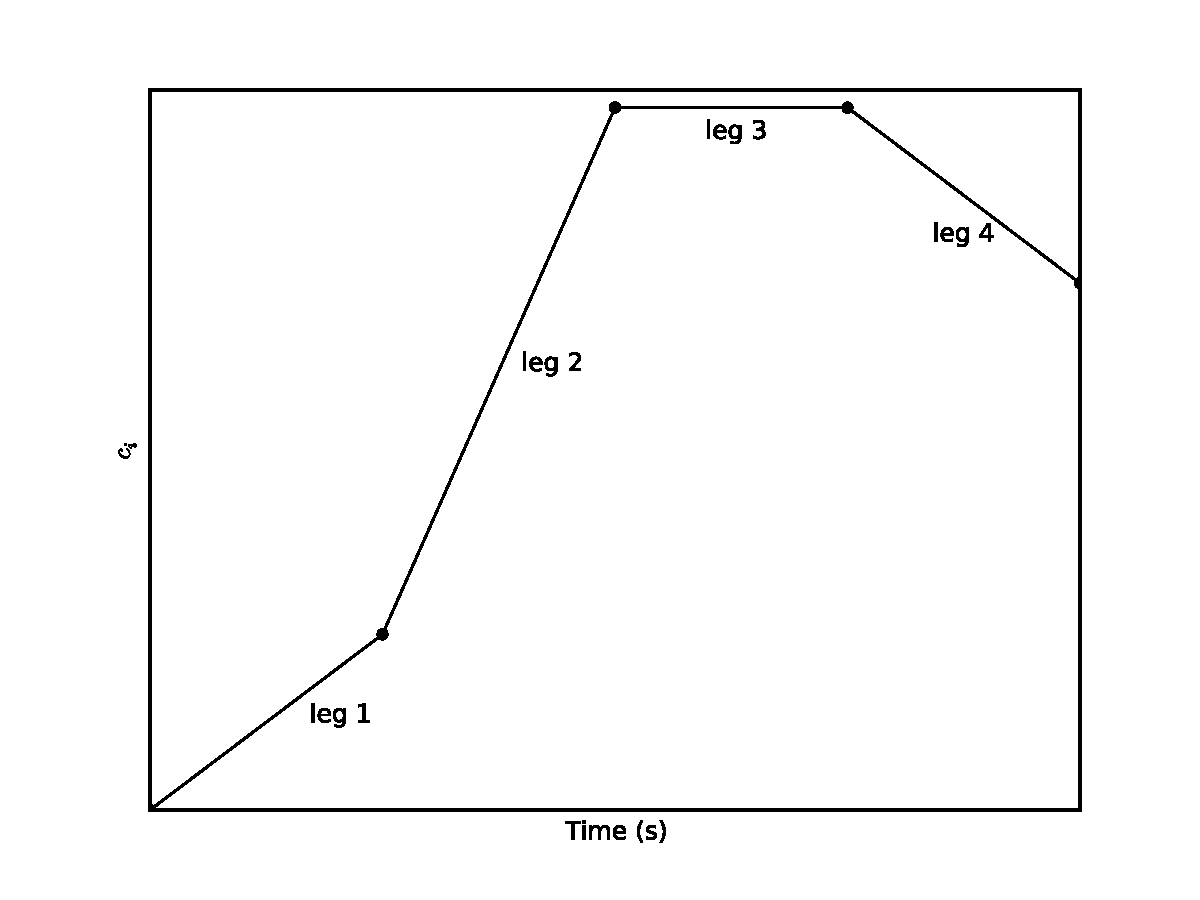
\includegraphics[width=.75\textwidth]{path.pdf}
  \caption{User defined path for the $i^{\text{th}}$ component of ``$c$''.
    $c$ may represent strain, strain rate, stress, stress rate, deformation
    gradient, displacement, or velocity.}
  \label{fig:path}
\end{figure}

The components of strain are defined by

\begin{equation}
  \Strain = \frac{1}{\kappa}\left(\RightStretch^\kappa - \SOIdentity\right)
\end{equation}
%
where $\RightStretch$ is the right Cauchy stretch tensor, defined by the polar
decomposition of the deformation gradient $\DefGrad =
\Rotation\DotProd\RightStretch$, and $\kappa$ is a user specified
``Seth-Hill'' parameter that controls the strain definition. Choosing
$\kappa=2$ gives the Lagrange strain, which might be useful when testing
models cast in a reference coordinate system. The choice $\kappa=1$, which
gives the engineering strain, is convenient when driving a problem over the
same strain path as was used in an experiment. The choice $\kappa=0$
corresponds to the logarithmic (Hencky) strain. Common values of $\kappa$ and
the associated names for each (there is some ambiguity in the names) are
listed in Table \ref{tab:kappa}.

\begin{table}[h]
  \label{tab:kappa}
  \centering
  \begin{tabular}{ll}
    \hline
    $\kappa$ &  Name(s) \\
    \hline
    -2 & Green \\
    -1 & True, Cauchy \\
     0 & Logarithmic, Hencky, True \\
     1 & Engineering, Swainger \\
     2 & Lagrange, Almansi \\
     \hline
  \end{tabular}
\end{table}

The volumetric strain $\Strain[v]$ is defined

\begin{equation}
  \label{eq:volstrain}
  \Strain[v] =
  \begin{cases}
    \OneOver{\kappa}\left(\Jacobian^{\kappa} - 1\right)
    & \text{if }\kappa \ne 0 \\
    \ln{\Jacobian} & \text{if }\kappa = 0
  \end{cases}
\end{equation}

where the Jacobian $\Jacobian$ is the determinant of the deformation gradient.

Each leg in the control table, from time $t=0$ to $t=t_f$ is subdivided into
a user-specified number of steps and the material model evaluated at each
step.  When volumetric strain, deformation gradient, displacement, or velocity
are specified for a leg, \mml{} internally determines the corresponding strain
components.  If a component of stress is specified, \mml{} determines the
strain increment that minimizes the distance between the prescribed stress
component and model response.

% ----------------------------------------------------------------------------- %
\subsection{Strain Rate from Prescribed Stress}
\label{sec:sig2d}
The approach to determining unknown components of the strain rate from the
prescribed stress is an iterative scheme employing a multidimensional Newton's
method that satisfies
%
\begin{displaymath}
  \Stress\left(\dStrain\,[\vc]\right) = \PrescStress
\end{displaymath}
%
where, $\vc$ is a vector subscript array containing the components for which
stresses (or stress rates) are prescribed, and $\PrescStress$ are the
components of prescribed stress.

Each iteration begins by determining the submatrix of the material
stiffness
\begin{displaymath}
  \Stiffness_{\vc} = \Stiffness\,[\vc, \vc]
\end{displaymath}
%
where $\Stiffness$ is the full stiffness matrix
$\Stiffness=d\Stress/d\Strain$. The value of $\dStrain\,[\vc]$ is then updated
according to
%
\begin{displaymath}
  \dStrain\,[\vc] = \dStrain\,[\vc] -
                   \Stiffness_{\vc}\DDotProd\Stress^{*}(\dStrain\,[\vc])/dt
\end{displaymath}
%
where
%
\begin{displaymath}
  \Stress^{*}(\dStrain\,[\vc]) = \Stress(\dStrain\,[\vc]) - \PrescStress
\end{displaymath}

The Newton procedure will converge for valid stress states.  However, it is
possible to prescribe invalid stress state, e.g.~a stress state beyond the
material's elastic limit.  In these cases, the Newton procedure may not
converge to within the acceptable tolerance and a Nelder-Mead simplex method
is used as a back up procedure.  A warning is logged in these cases.

% ----------------------------------------------------------------------------- %
\subsection{Solid Driver}
\label{sec:solid-driver}
As the name implies, the \sol{} driver is designed to exercise the type of
material models encountered in solid mechanics. The solution method is similar
to that of many finite element codes, so that material models developed and
tested in \mml{} can be easily transitioned to them.

% ----------------------------------------------------------------------------- %
\subsection{Electrical}
\label{sec:elec}
Electric field can be prescribed for testing piezoelectric models.

% ----------------------------------------------------------------------------- %
\chapter{Running Simulations in \mml{}}
\label{chap:run}
The command line utility \mmd{} is the main program with which users interact
with \mml{}. To run a simulation with \mml{}, be sure that \verb|$MMLROOT| is
on your path and execute

\begin{verbatim}
$ mmd runid[.xml]
\end{verbatim}
%
where \texttt{runid} is the basename of the input file. Input file
formatting is covered in Chapters \ref{chap:inpov} - \ref{chap:inpopt}.

The following files will be produced by \mmd{} in the current working
directory
\begin{verbatim}
$ ls runid.*
runid.exo       runid.log       runid.xml
\end{verbatim}
%
\texttt{runid.exo} is the \exodusii{} output database, \texttt{runid.log} the
log file, and \texttt{runid.xml} the input file.

For a complete list of options, execute
\begin{verbatim}
$ mmd -h
\end{verbatim}


% ----------------------------------------------------------------------------- %
\chapter{User Input: Overview}
\label{chap:inpov}
User input is via xml control files. In general, tags use CamelCase and
attributes lower case.  Attributes are described in this document as
%
\begin{verbatim}
attr="type[default]{choices}"
\end{verbatim}
%
where \texttt{default} is the default value (if any) and \texttt{\{choices\}}
are valid choices (if any). Any attribute not having a default value is
required. Types are \texttt{str}, \texttt{int}, \texttt{real}, \texttt{list}
and \texttt{boolean}. Lists are given as space separated lists (e.g., "1 2
3"), boolean arguments should be true or false.

In the following, elements shown in \Red{red} are required input.

% ----------------------------------------------------------------------------- %
\section{\reqdtag{MMLSpec}}
\label{sec:mmlspec}
All input files must have as their root element \reqdtag{MMLSpec}.
\begin{inpusage}
<MMLSpec>
\end{inpusage}

Recognized subelements of \reqdtag{MMLSpec} are
%
\begin{itemize}
  \item \reqdtag{Physics}
  \item \tag{Permutation}
  \item \tag{Optimization}
\end{itemize}

The following elements are read from any scope in the input file
%
\begin{itemize}
  \item \tag{Include}
  \item \tag{Function}
\end{itemize}

The \reqdtag{Physics}, \tag{Permutation}, \tag{Optimization} and input blocks
are described separately in their own chapters.

% ----------------------------------------------------------------------------- %
\section{Preprocessing}
\label{sec:pre}
Preprocessing allows specifying variables in the input inside of comment tags
for use in other parts of the input. Syntax mirrors that of \texttt{aprepro}.
Preprocessor also evaluates (nearly) any Python expression.

The \texttt{random()} expression generates a random number. The
\verb|random_seed| variable sets the random state seed. Note, expressions are
evaluated in order, therefore, if setting the \verb|random_seed| it should
occur early.

The following input stub demonstrates specifying the \reqdtag{Material}
parameter \texttt{K} and \texttt{G}, and \tag{Path} parameter \texttt{estar}
as variables
\begin{example}
<MMLSpec>
  <!-- {random_seed = 7}
       {G = 54e9 * random()}
       {K = 23e9}
       {estar = -.05}
  -->
  <Physics>
    <Material model="elastic">
      <K> {K} </K>
      <G> {G} </G>
    </Material>
    <Path type="prdef" estar="{estar}">
      ...
    </Path>
  </Physics>
</MMLSpec>
\end{example}

% ----------------------------------------------------------------------------- %
\section{\tag{Include}}
\label{sec:inc}
Path to file to be included as if its contents were inplace in the input file

\begin{inpusage}
<Include href="str"/>
\end{inpusage}

The following stub input demonstrates how to include a file in place
\begin{example}
<Include href="/path/to/some/file.ext"/>
\end{example}

% ----------------------------------------------------------------------------- %
\section{\tag{Function}}
\label{sec:func}
Define functions to be used elsewhere in input. \texttt{id=0} and
\texttt{id=1} are reserved for the constant $0$ and $1$ functions,
respectively. \attr{href} is the path to a file containing the function
definition (useful when the function is a large piecewise linear table).
\attr{cols} specifies the columns in which data is located in a piecewise
linear table.

\begin{inpusage}
<Function id="int"
          type="str{analytic_expression, piecewise_linear}"
          var="str[x]" href="str[]" cols="list[1 2]">
\end{inpusage}

The following input stub demonstrates how to define an analytic expression and
piecewise linear table as functions

\begin{example}
<Function id="2" type="analytic_expression" var="t">
  sin(t)
</Function>
<Function id="3" type="piecewise_linear">
  1 2
  2 3
  3 5
</Function>

<!-- Read a piecewise linear table from an external file using
     columns 1 and 3
-->
<Function id="4" type="piecewise_linear" href="./file.dat"
          cols="1 3"/>
\end{example}

\begin{verbatim}
$ cat file.dat
# Column1 Column2 Column3
1 1 4
2 3 7
.
.
.
100 4.2 1.43
\end{verbatim}

% ----------------------------------------------------------------------------- %
\chapter{User Input: \reqdtag{Physics}}
\label{chap:inpphys}
Define the physics of the simulation.

\begin{inpusage}
<Physics driver="str[solid]{solid, eos}"
         termination_time="real[]" runid="str[filename]">
\end{inpusage}

Recognized subelements of \reqdtag{Physics} are
%
\begin{itemize}
  \item \reqdtag{Path}
  \item \reqdtag{Material}
  \item \tag{Extract}
\end{itemize}


% ----------------------------------------------------------------------------- %
\section{\reqdtag{Physics} Attributes}
\label{sec:phys-attr}

% ----------------------------------------------------------------------------- %
\subsection{\attr{driver}}
\label{sec:driv-attr}
\attr{driver} specifies the driver type to use.  Defaults to \texttt{solid}.

\subsection{\attr{termination\_time}}
\label{sec:tterm-attr}
If specified, \verb:termination_time: defines the termination time for the
simulation. If not specified, termination time is taken as final time in
\reqdtag{Path}.

\subsection{\attr{runid}}
\label{sec:tterm-attr}
If specified, \texttt{runid} redefines the \texttt{runid} from its default
\texttt{basename(file)}.


% ----------------------------------------------------------------------------- %
\section{\reqdtag{Path}}
\label{sec:path-attr}
Define deformation paths through with the material will be exercised.

\begin{inpusage}
<Path type="str{prdef, surface}"
      format="str[default]{default, table, fcnspec}"
      cols="list[1, ..., n]" cfmt="str"
      tfmt="str[time]{time,dt}"
      nfac="int[1]" kappa="real[0]" rstar="real[1]"
      tstar="real[1]" estar="real[1]" sstar="real[1]"
      amplitude="real[1]" ratfac="real[1]" href="str">
\end{inpusage}

% ----------------------------------------------------------------------------- %
\subsection{\reqdtag{Path} Attributes}
\label{sec:path}

% ----------------------------------------------------------------------------- %
\subsubsection{\attr{type}}
\label{sec:path-type}
The type of path specified.  Valid types are \texttt{prdef} and
\texttt{surface}.

The \texttt{prdef} type defines a prescribed deformation. The jth leg of
\reqdtag{Path} is sent to the driver in form \texttt{[tf, n, cfmt, Cij]},
where \texttt{tf}, \texttt{n}, \texttt{cfmt}, and \texttt{Cij} are the
termination time, number of steps, control format, and control values. Methods
of inputing legs depends on the attributes of \reqdtag{Path} and will be shown
in examples to follow.

The \texttt{surface} input is similar to the \texttt{prdef} specification, but
leg termination time is not specified. Control parameters also differ, as
shown in Table \ref{tab:cfmt-1}.

% ----------------------------------------------------------------------------- %
\subsubsection{\attr{format}}
\label{sec:path-format}
The format by which the legs of the deformation path are specified. Valid
formats are \texttt{default}, \texttt{table}, and \texttt{fcnspec}. In the
following subsections, the different formats are described.

% ----------------------------------------------------------------------------- %
\paragraph{\attr[default]{format}}
\label{sec:defform}
The \texttt{default} format offers the most control.  In this format, the
termination time, number of steps, control format, and components of
deformation are specified for each leg as in the following stub input

\begin{example}
<Path type="default">
  <!-- tterm nsteps cfmt c1 c2 c3 ... -->
  0  0 222222 0 0 0 0 0 0
  1 10 222222 1 0 0 0 0 0
</Path>
\end{example}

See Section \ref{sec:cfmt} for a full description of the control format
\texttt{cfmt} and its relationship with the \texttt{c1, c2, c3, ...}.

% ----------------------------------------------------------------------------- %
\paragraph{\attr[table]{format}}
\label{sec:tblform}
The \texttt{table} format allows reading in deformation paths from a columnar
table of data. Control format is uniform for all legs. Specify control format
as \texttt{cfmt} attribute of \reqdtag{Path}. Specify which columns to read
data with the \texttt{cols} attribute. The first column is assumed to be the
time specifier. See Section \ref{sec:colspec} for a description of the
\texttt{cols} attribute. The \texttt{tfmt} attribute specifies if the time
column represents the actual time (\verb|tfmt="time"|) or time step
(\texttt{tmft="dt"}). The number of steps for each leg can be set by
\texttt{nfac}. The \texttt{href} attribute specifies an external file to read
the table.

The following input stubs demonstrate reading a table from the input file and
from an external file.

\begin{example}
<!-- Read entries from table. -->
<Path type="prdef" format="table" cols="1:4" cfmt="222"
      tfmt="time">
  0 0 0 0
  1 1 0 0
    ...
  n 2 0 0
</Path>
\end{example}

\begin{example}
<!-- Read table from external file -->
<Path type="prdef" format="table" cols="1 3:8" cfmt="222222"
      tfmt="time" href="exmpls.tbl"/>
\end{example}

% ----------------------------------------------------------------------------- %
\paragraph{\attr[fcnspec]{format}}
\label{sec:fcnspec}
The \texttt{fcnspec} format allows defining a deformation path by a function.
A deformation path defined by \texttt{fcnspec} must have only 1 leg defining
the termination time and the function specifier defining the values of the
components of deformation.  The function specifier is of the form

\begin{example}
function_id[:scale]
\end{example}

\noindent where \texttt{function\us{}id} is the ID of the function as
specified in its \tag{Function} element. The optional scale is multiplied by
the function.

The following input stub demonstrates uniaxial strain deformation, using a
user defined function to specify the 11 component of strain through time.

\begin{example}
<Path type="prdef" format="fcnspec" cfmt="222" nfac="200">
  <!-- termination time, fcn spec -->
  {2 * pi} 2:1.e-1 0 0
</Path>
\end{example}

% ----------------------------------------------------------------------------- %
\subsubsection{\attr{cfmt}}
\label{sec:cfmt}
The control format \texttt{cfmt} is concatenated integer list specifying in
its $i^\text{ith}$ component the $i^\text{th}$ component of deformation, i.e.,
\texttt{cfmt[i]} instructs the driver as to the type of deformation
represented by \texttt{Cij[i]}. Types of deformation represented by
\texttt{cfmt} are shown in Table \ref{tab:cfmt} for the \sol{} driver and
Table \ref{tab:cfmt-1} for the \eos{} driver.

For example, the following \texttt{cfmt} instructs the driver that the
components of \texttt{Cij} represent [stress, strain, stress rate, strain
rate, strain, strain], respectively:

\begin{example}
cfmt="423122"
\end{example}

Mixed modes are allowed only for components of strain rate, strain, stress
rate, and stress. Electric field components can be included with any
deformation type.  If only one component of stress rate, stress, strain rate,
or strain is specified, the component \texttt{Cij} is taken to be either the
pressure of volumetric strain.

The components \texttt{Cij} take the following order

\paragraph{Vectors:} [X, Y, Z]

\paragraph{Symmetric tensors:} [XX, YY, ZZ, XY, YZ, XZ]

\paragraph{Tensors:} [XX, XY, XZ, YX, YY, YZ ZX, ZY, ZZ]

If \texttt{len(Cij) $\neq$ 6} (or 9 for deformation gradient), the missing
components are assumed to be zero strain.

\begin{table}[h!]
  \centering
  \begin{tabular}[h]{cl}
    \hline
    \hline
    \texttt{cfmt} & Deformation type \\
    \hline
    1 & Strain rate \\
    2 & Strain \\
    3 & Stress rate \\
    4 & Stress \\
    5 & Deformation gradient \\
    6 & Electric field
  \end{tabular}
  \caption{Supported deformation types and \texttt{cfmt} code for
    \texttt{solid} \texttt{prdef} paths}
  \label{tab:cfmt}
\end{table}

\begin{table}[h!]
  \centering
  \begin{tabular}[h]{cl}
    \hline
    \hline
    \texttt{cfmt} & Variable type \\
    \hline
    1 & Density \\
    2 & Temperature
  \end{tabular}
  \caption{Supported surface variable types and \texttt{cfmt} code for
    \texttt{eos} \texttt{surface} paths}
  \label{tab:cfmt-1}
\end{table}

% ----------------------------------------------------------------------------- %
\subsubsection{\attr{tfmt}}
\label{sec:tfmt}
The \texttt{tfmt=["time"]\{"time","dt"\}} flag specifies the time format.
If \texttt{tfmt="time"} (default) the first value of each leg is interpreted
as the termination time for the leg. For \texttt{tfmt="dt"} the first value
of each leg is interpreted as a time increment.

% ----------------------------------------------------------------------------- %
\subsubsection{\attr{cols}}
\label{sec:colspec}
The columns to be read from a table or the \texttt{fcnspec} leg are specified by
the \texttt{cols} attribute.  \texttt{cols} are specified as a space separated
list of columns.  Numbering is 1 based.  Ranges can be specified using Python
slice syntax.

The following input stubs demonstrate two equivalent ways to to read columns
1, 3, 4, 5, 8, 9, and 13 from a table.
\begin{example}
cols="1 3 4 5 8 9 13"
\end{example}

\begin{example}
cols="1 3:5 8:9 13"
\end{example}

% ----------------------------------------------------------------------------- %
\subsubsection{\attr{kappa}}
\label{sec:kappa}
\texttt{kappa} is the Seth-Hill strain definition parameter $\kappa$ described
in section \ref{sec:mmlsol}.

% ----------------------------------------------------------------------------- %
\subsubsection{\attr{nfac}}
\label{sec:nfac}
\texttt{nfac} is a multiplier on the number of steps for each leg.

% ----------------------------------------------------------------------------- %
\subsubsection{\attr{amplitude}}
\label{sec:ampl}
\texttt{amplitude} is a factor multiplied to all components of deformation.

% ----------------------------------------------------------------------------- %
\subsubsection{The ``star'' Multipliers}
\label{sec:stars}
\texttt{[rtes(ef)]star} are multipliers on the components of density, time
(temperature for \texttt{type="surface"}), strain, stress, and electric field,
respectively. The \texttt{[rtes(ef)]star} are first multiplied by
\texttt{amplitude}.

% ----------------------------------------------------------------------------- %
\subsubsection{\attr{ratfac}}
\label{sec:ratfac}
\texttt{ratfac} is a divisor to the termination time of each leg, thereby
effectively increasing the rate of deformation.

% ----------------------------------------------------------------------------- %
\subsection{More Examples}
\label{sec:more-ex}
The following examples will help clarify the \reqdtag{Path} input syntax

\begin{example}
<!-- uniaxial strain, all six components of strain
     prescribed -->
<Path type="prdef" kappa="0" tstar="1" estar="-.5"
      amplitude="1" ratfac="1">
  <!-- termination time, number of steps, cfmt, Cij -->
  0   0 222222 0 0 0 0 0 0
  1 100 222222 1 0 0 0 0 0
  2 100 222222 2 0 0 0 0 0
  3 100 222222 1 0 0 0 0 0
  4 100 222222 0 0 0 0 0 0
</Path>
\end{example}

\begin{example}
<!-- uniaxial strain, stress controlled -->
<Path type="prdef" nfac="100">
  0 0 444 0 0 0
  1 1 444 -7490645504 -3739707392 -3739707392
  2 1 444 -14981291008 -7479414784 -7479414784
  3 1 444 -7490645504 -3739707392 -3739707392
  4 1 444 0 0 0
</Path>
\end{example}

\begin{example}
<!-- uniaxial stress, mixed mode -->
<Path type="prdef" nfac="100">
  0 0 222 0 0 0
  1 1 244 {epsmax} 0 0
  4 1 244 0 0 0
</Path>
\end{example}

\begin{example}
<!-- volumetric strain -->
<Path type="prdef" kappa="0" estar="-.5">
  0   0 2 0
  1 100 2 1
  2 100 2 2
  3 100 2 1
  4 100 2 0
</Path>
\end{example}

\subsubsection{Example of \attr[surface]{type}}
\label{sec:more-ex-1}
The following examples demonstrate the \texttt{type="surface"}
\begin{example}
<Path type="surface">
  <!-- nsteps, control, Cij -->
  <!-- control goes as 1 -> density
                       2 -> temperature -->
    0 12 1 100
  100 12 5 300
</Path>
\end{example}

\begin{example}
<Path type="surface" format="table" cfmt="12" nfac="100">
  <!-- Cij -->
  1 100
  5 300
</Path>
\end{example}

% ----------------------------------------------------------------------------- %
\section{\reqdtag{Material}}
\label{sec:mtl}
Define the material model.

\begin{inpusage}
<Material model="str" constant_jacobian="boolean[false]">
\end{inpusage}

Subelements of \reqdtag{Material} are
%
\begin{itemize}
  \item \tag{Matlabel}
  \item \tag{ParameterArray}
  \item \tag{InitialState}
  \item \tag{Key}*
\end{itemize}
%
*\tag{Key} is a valid material parameter name.

% ----------------------------------------------------------------------------- %
\subsection{\reqdtag{Material} Attributes}
\label{sec:mtl-attr}

% ----------------------------------------------------------------------------- %
\subsubsection{\attr{model}}
\label{sec:model}
The name of the material model.

% ----------------------------------------------------------------------------- %
\subsubsection{\attr{constant\_jacobian}}
\label{sec:constjac}
Use the initial (constant) jacobian during inverse stress driven problems.

% ----------------------------------------------------------------------------- %
\subsection{\tag{Matlabel}}
\label{sec:matlabel}
Insert model parameters from a database file.
\begin{inpusage}
<Matlabel href="str[F_MTL_PARAM_DB]" material="str"/>
\end{inpusage}

% ----------------------------------------------------------------------------- %
\subsubsection{\tag{Matlabel} Attributes}
\label{sec:matlabel-attr}
\paragraph{\attr{href}}
The path to the database file. Defaults to\\
\verb:$MMLROOT/materials/material_properties.db: if no file is given.

% ----------------------------------------------------------------------------- %
\paragraph{\attr{material}}
Name of material as given in the database file.

The following input stub demonstrates the use of \tag{Matlabel}
\begin{example}
<Material model="elastic">
  <Matlabel href="./materials.xml" material="aluminum"/>
</Material>
\end{example}

\subsection{\tag{ParameterArray}}
\label{sec:param-array}
Specify the parameter array for the material as whitespace separated list of
floats.  The list of values must be the same length as the parameter array for
the material or an error will occur.
\begin{inpusage}
<ParameterArray>
  VAL1 VAL2 ... VALN
</ParameterArray>
\end{inpusage}

% ----------------------------------------------------------------------------- %
\subsection{\tag{InitialState}}
\label{sec:initial-state}
Specify the initial state of the material as a whitespace separated list of
floats. Six stress values must be followed by material variables (if any). The
length of the material variables must be the same as the length of the
\texttt{xtra} variable array for the material or an error will occur.  Note,
implementation is material model specific.
\begin{inpusage}
<InitialState>
  STRESS_XX STRESS_YY ... STRESS_XZ XTRA1 XTRA2 ... XTRAN
</InitialState>
\end{inpusage}

% ----------------------------------------------------------------------------- %
\subsection{Specify Individual Parameters}
\label{sec:ind-params}
Specify individual parameters as xml text nodes
\begin{inpusage}
<Key> float </Key>
\end{inpusage}

\tag{Key} is replaced by specific material model parameters. The following
stub inputs demonstrate the \reqdtag{Material} input
\begin{example}
<Material model="elastic">
  <G>  54E+09 </G>
  <K> 124E+09 </K>
</Material>
\end{example}

% ----------------------------------------------------------------------------- %
\section{\tag{Extract}}
\label{sec:extract}
Extract variables and paths from \exodusii{} output and (optionally) write to
different formats.
\begin{inpusage}
<Extract format="str[ascii]{ascii, mathematica, ndarray}"
         step="int[1]" ffmt="str[.18f]">
\end{inpusage}

Recognized subelements of \tag{Extract} are
%
\begin{itemize}
  \item \tag{Path}*
  \item \tag{Variables}
\end{itemize}
%
* \texttt{eos} driver only

% ----------------------------------------------------------------------------- %
\subsection{\tag{Extract} Attributes}
\subsubsection{\attr{format}}
The format to write the output.  \texttt{ascii} format writes out columnar
data as an ascii text file, \texttt{mathematica} writes an ascii text file
that can be read by Mathematica, and \texttt{ndarray} writes the data to a
file in the numpy .npy binary format.

% ----------------------------------------------------------------------------- %
\subsubsection{\attr{step}}
\label{sec:step}
Extract every \texttt{step}th timestep.

% ----------------------------------------------------------------------------- %
\subsubsection{\attr{ffmt}}
\label{sec:ffmt}
The string format used write out variables.

% ----------------------------------------------------------------------------- %
\subsection{\tag{Variables}}
\label{sec:vars}
Variables to extract from the \exodusii{} output database. Variables are specified
children of the \tag{Variables} element. All components of vector and tensor
variables will be extracted if only the basename is specified. Time is always
extracted as the first entry of the output file.  Extracted variables are in
\texttt{runid.out} or \texttt{runid.math} depending if the format is ascii or
mathematica.
\begin{inpusage}
<Variables>
  VAR_1, ..., VAR_N
</Variables>
\end{inpusage}

The following example demonstrates how to extract all components of stress and
strain
\begin{example}
<Extract format="ascii">
  <variables>
    STRESS STRAIN
  </variables>
</Extract>
\end{example}

Extract only the XX, YY, and ZZ components of stress
\begin{example}
<Extract format="ascii">
  <variables>
    STRESS_XX STRESS_YY STRESS_ZZ
  </variables>
</Extract>
\end{example}

Extract all variables
\begin{example}
<Extract format="ascii">
  <variables>
    ALL
  </variables>
</Extract>
\end{example}

% ----------------------------------------------------------------------------- %
\subsubsection{\tag{Path}}
\label{sec:vars-path}
Extract a specified path from the equation of state surface through the
specified density range starting at the initial temperature.
\begin{inpusage}
<Path type="str{isotherm, hugoniot}" increments="int[100]"
      density_range="list" initial_temperature="real">
\end{inpusage}

The following input stub demonstrates extracting Hugoniot and Isotherm paths
\begin{example}
<Extract>
  <Path type="isotherm" increments="200"
        density_range="1 3" initial_temperature="225"/>
  <Path type="hugoniot" increments="100"
        density_range="1 3" initial_temperature="100"/>
</Extract>
\end{example}

% ----------------------------------------------------------------------------- %
\chapter{User Input: \tag{Permutation}}
\label{chap:inpperm}
Permutate model input parameters, running jobs with different realization of
parameters. Ideal for investigating model sensitivities.
%
\begin{inpusage}
<Permutation method="str[zip]{zip,combine,shotgun}"
                     seed="real[date]"
                     correlation="list[none]{plot,table,none}">
\end{inpusage}

Recognized subelements of \tag{Permutation} are

\begin{itemize}
  \item \reqdtag{Permutate}
  \item \tag{ResponseFunction}
\end{itemize}

Each \tag{Permutation} job creates a directory \texttt{runid.eval}
\begin{verbatim}
$ ls runid.eval
eval_0/    eval_2/    mml-evaldb.xml
eval_1/    ...        runid.log
\end{verbatim}

The \texttt{eval\us{}i} directory holds the output of the
\texttt{i}$^{\text{th}}$ job, including \texttt{params.in} with the values of
each permutated parameter for that job. \texttt{mml-tabular.xml} contains a
summary of each job run. \mmv{} recognizes \texttt{mml-tabular.xml} files.

% ----------------------------------------------------------------------------- %
\section{\tag{Permutation} Attributes}
\label{sec:perm-attr}

% ----------------------------------------------------------------------------- %
\subsection{\attr{method}}
\label{sec:perm-meth}
The \texttt{method} attribute describes which method to use to determine
parameter combinations to run.

The \texttt{zip} method runs one job for each set of parameters (and, thus,
the number of realizations for each parameter must be identical), the
\texttt{combine} method runs every combination of parameters.

% ----------------------------------------------------------------------------- %
\subsection{\attr{correlation}}
\label{sec:perm-corr}
Create correlation table and plots of relating permutated parameters and value
of response function. \texttt{correlation} is only meaningful if a
\tag{ResponseFunction} is specified.

% ----------------------------------------------------------------------------- %
\subsection{\attr{seed}}
\label{sec:perm-seed}
The seed for the random number generator. \texttt{date} is todays date in
seconds.

% ----------------------------------------------------------------------------- %
\section{\tag{Permutate}}
\label{sec:permutate}
Specify the paramaters to permutate.
\begin{inpusage}
<Permutate var="str"
           values="func{range,list,weibull,uniform,
                        normal,percentage}"
\end{inpusage}

% ----------------------------------------------------------------------------- %
\subsection{\tag{Permutate} Attributes}
\label{sec:permutate-attr}

% ----------------------------------------------------------------------------- %
\subsubsection{\attr{var}}
\label{perm-var}
\texttt{var} is the name of the variabe and should occur elsewhere in
the input file in preprocessing braces.

% ----------------------------------------------------------------------------- %
\subsubsection{\attr{values}}
\label{sec:perm-vals}
\texttt{values} are the specific values. The
\texttt{range,list,weibull,uniform,normal,percentage} are all specified as
functions with the following form

\begin{example}
values="func(start,stop,N)"
\end{example}

The following input stub demonstrates how to permutate the \texttt{K} and
\texttt{G} parameters
%
\begin{example}
<Permutation method="zip" seed="12">
  <Permutate var="K" values="weibull(125.e9, 14, 3)"/>
  <Permutate var="G" values="percentage(45.e9, 10, 3)"/>
</Permutation>
\end{example}

In the \tag{Material} element, the \texttt{K} and \texttt{G} parameters are
specified as
%
\begin{example}
<Material model="elastic">
  <K> {K} </K>
  <G> {G} </G>
</Material>
\end{example}

% ----------------------------------------------------------------------------- %
\section{\tag{ResponseFunction}}
\label{sec:perm-resp-func}
The \tag{ResponseFunction} returns the response from permutation or
optimization jobs.
\begin{inpusage}
<ResponseFunction href="str" function="mmlfcn"
                  descriptor="str[]"/>
\end{inpusage}

One of \texttt{href} or \texttt{function} must be specified.

% ----------------------------------------------------------------------------- %
\subsection{\tag{ResponseFunction} Attributes}
\label{sec:perm-resp-func-attr}

% ----------------------------------------------------------------------------- %
\subsubsection{\attr{descriptor}}
\label{sec:perm-resp-func-attr-desc}
\texttt{descriptor} is the name given to the response function in the output.

% ----------------------------------------------------------------------------- %
\subsubsection{\attr{href}}
\label{sec:perm-resp-func-attr-href}
\texttt{href} is the path to an executable file script containing the response
function. The script is called from the command line as

\begin{verbatim}
% ./scriptname runid.exo
\end{verbatim}

An example of a response function specifying \texttt{href} is
\begin{example}
<ResponseFunction href="./scriptname" descriptor="PRES"/>
\end{example}

% ----------------------------------------------------------------------------- %
\subsubsection{\attr{function}}
\label{sec:perm-resp-func-attr-fcn}
\texttt{function} is the name of a builtin \mml{} response function. Built in
response functions are
%
\begin{itemize}
  \item \texttt{mml.max} maximum value of a simulation variable output
  \item \texttt{mml.min} minimum value of a simulation variable output
  \item \texttt{mml.mean} mean value of a simulation variable output
  \item \texttt{mml.ave} average value of a simulation variable output
  \item \texttt{mml.absmax} maximum absolute value of a simulation variable output
  \item \texttt{mml.absmin} minimum absolute value of a simulation variable output
\end{itemize}
%
Built in response functions operate only on variabes in the simulation output file.

An example of a response function specifying \texttt{function} is
\begin{example}
<ResponseFunction function="mml.max(PRESSURE)"
                  descriptor="PRES"/>
\end{example}

% ----------------------------------------------------------------------------- %
\chapter{User Input: \tag{Optimization}}
\label{chap:inpopt}
Optimize specified parameters against user specified objective function.
%
\begin{inpusage}
<Optimization method="str[simplex]{simplex, powell, cobyla}"
              maxiter="int[25]" tolerance="real[1e-6]">
\end{inpusage}

Recognized subelements of \tag{Optimization} are

\begin{itemize}
  \item \reqdtag{Optimize}
  \item \reqdtag{ResponseFunction}
  \item \tag{AuxiliaryFile}
\end{itemize}

Like \tag{Permutation} jobs, each \tag{Optimization} job creates a directory
\texttt{runid.eval}
\begin{verbatim}
$ ls runid.eval
eval_0/    eval_2/    mml-evaldb.xml     runid.log
eval_1/    ...        params.opt
\end{verbatim}

The \texttt{eval\us{}i} directory holds the output of the
\texttt{i}$^{\text{th}}$ job, including \texttt{params.in} with the values of
each parameter for that job. \texttt{mml-tabular.xml} contains a
summary of each job run. \mmv{} recognizes \texttt{mml-tabular.xml} files.
\texttt{params.opt} has the final, optimized, parameters.

% ----------------------------------------------------------------------------- %
\section{\tag{Optimization} Attributes}
\label{sec:opt}

% ----------------------------------------------------------------------------- %
\subsection{\attr{method}}
\label{sec:opt-meth}
\texttt{method} specifies the optimization method.  All optimization routines
utilize the scipy.optimize module.

% ----------------------------------------------------------------------------- %
\subsection{\attr{maxiter}}
\label{sec:maxiter}
\texttt{maxiter} is the maximum number of iterations.

% ----------------------------------------------------------------------------- %
\subsection{\attr{tolerance}}
\label{sec:tol}
\texttt{tolerance} is the optimization tolerance.

% ----------------------------------------------------------------------------- %
\section{\tag{Optimize}}
\label{sec:optimize}
Specify the variable to be optimized.
\begin{inpusage}
<Optimize var="str" initial_value="real" bounds="list[]"/>
\end{inpusage}

% ----------------------------------------------------------------------------- %
\subsection{\tag{Optimize} Attributes}
\label{sec:optimize-attr}

% ----------------------------------------------------------------------------- %
\subsubsection{\attr{var}}
\label{sec:optimize-attr-val}
\texttt{var} is the name of the variabe and should occur elsewhere in
the input file in preprocessing braces.

% ----------------------------------------------------------------------------- %
\subsubsection{\attr{initial\_value}}
\label{sec:optimize-attr-ival}
\texttt{initial\us{}value} is the initial value of \texttt{var}

% ----------------------------------------------------------------------------- %
\subsubsection{\attr{bounds}}
\label{sec:optimize-attr-bounds}
\texttt{bounds} specifies lower and upper bounds on \texttt{var}. Only the
\texttt{cobyla} method accepts bounds.

% ----------------------------------------------------------------------------- %
\section{\tag{AuxiliaryFile}}
\label{sec:optimize-aux-file}
Path to any auxiliary file needed by the optimization objective function.
\begin{inpusage}
<AuxiliaryFile href="str"/>
\end{inpusage}

% ----------------------------------------------------------------------------- %
\section{\reqdtag{ResponseFunction}}
\label{sec:optimize-resp-fcn}
Same as for \tag{Permutation}, except that auxiliary files are also passed to
the function. The value returned from the response function is interpreted as
the error to be minimized.

If the \tag{ResponseFunction} is given by \texttt{href}, it is called as
\begin{verbatim}
% ./scriptname runid.exo [AuxFile1[AuxFile2[...]]]
\end{verbatim}

% ----------------------------------------------------------------------------- %
\section{Example}
\label{sec:optimize-ex}
Optimize the \texttt{K} and \texttt{G} parameters
\begin{example}
<Optimization method="simplex" maxiter="25" tolerance="1e-4">
  <ResponseFunction href="opt-sig-v-time"
                    descriptor="SIG_V_TIME"/>
  <AuxiliaryFile href="opt-baseline.dat"/>
  <Optimize var="opt_k" initial_value="129.e9"/>
  <Optimize var="opt_g" initial_value="54.e9"/>
</Optimization>
\end{example}

In the \reqdtag{Material} element, the \texttt{K} and \texttt{G} parameters
are specified as
%
\begin{example}
<Material model="elastic">
  <K> {opt_k} </K>
  <G> {opt_g} </G>
</Material>
\end{example}

% ----------------------------------------------------------------------------- %
\chapter{User Material Interface}
\label{chap:usrmtl}
\mml{} can be made to find, build, and execute user materials outside of
\verb|$MMLROOT|.  User materials can be written in Python or Fortran and and
\mml{} interacts with them through the application programming interface
(API).  In general, the following pattern is followed for exercising a
material model with \mml{}:
%
\begin{enumerate}
  \item create a material model interface (MMI)
  \item build and link the material model to \mml{}
  \item exercise the model
\end{enumerate}
%

% ----------------------------------------------------------------------------- %
\section{Material Model Interface}
\label{sec:usrint}
\mml{} interacts with materials through a material interface file. The
material interface file defines the material class which must be a subclass of\\
\verb|$MMLROOT/materials._material.Material|.  In this section, methods of the
\verb|Material| class are described.

% ----------------------------------------------------------------------------- %
\subsection{Material Class Instantiation}
\label{sec:basecls}
The base class \verb|Material| in \verb|$MMLROOT/materials._material| creates
new \mml{} materials and provides the interface with which \mml{} interacts.
Each class must define its name (\verb|Material.name|) and an ordered list of
material parameter names (\verb|Material.param_names|) as they appear in the
input file.  The class should not define an \texttt{\uus{}init\uus{}} method
and if it does, should call the \texttt{\uus{}init\uus{}} of the base class.

\begin{interface}
  \textbf{Material: Interface}
\end{interface}
\usage{mtl = Material()}

The following is an example of a \texttt{Material} declaration for the
\texttt{Elastic} material model
%
\begin{example}
from materials._material import Material
class Elastic(Material)
    name = 'elastic'
    param_names = ['K', 'G']
\end{example}

% ----------------------------------------------------------------------------- %
\subsection{Setup the Material}
\label{sec:setup-mtl}
The method \texttt{setup} sets up the material model by checking and setting
the material parameter array, requesting allocation of storage of material
variables, and computing and storing the \verb|bulk_modulus| and
\verb|shear_modulus| of the material.

\begin{interface}
  \textbf{Material.setup: Interface}
\end{interface}
\usage{mtl.setup(params)}\\[5pt]
\param{ndarray params}{Material parameters parsed from the input file}

The following is an example of a \texttt{setup} method

\begin{example}
def setup(self, params):
    if elastic is None:
        raise Error1("elastic model not imported")
    elastic.elastic_check(params, log_error, log_message)
    K, G, = params
    self.set_param_vals(params)
    self.bulk_modulus = K
    self.shear_modulus = G
\end{example}

% ----------------------------------------------------------------------------- %
\subsection{Storing the Parameter Array}
\label{sec:store-param}
The method \verb|set_param_vals| stores the checked parameter values with
\mml{}.  It must be called by each instance of the material model.

\begin{interface}
  \textbf{Material.set\us{}param\us{}vals: Interface}
\end{interface}
\usage{mtl.set\us{}param\us{}vals(params)}\\[5pt]
\param{ndarray params}{Checked material parameters}

The following is an example of how \verb|set_param_vals| is used within a
mterials \verb|setup| method.

\begin{example}
params = self._check_params(params)
self.set_param_val(params)
\end{example}

% ----------------------------------------------------------------------------- %
\subsection{Adjust the Initial State}
\label{sec:adjust-istate}
The method \texttt{adjust\us{}initial\us{}state} adjusts the initial state
after the material is setup. Method provided by base class should be adequate
for most materials. A material should only overide the base method if
absolutely necessary.

\begin{interface}
  \textbf{Material.adjust\us{}initial\us{}state: Interface}
\end{interface}
\usage{mtl.adjust\us{}initial\us{}state(xtra)}\\[5pt]
\param{ndarray xtra}{Material variables}

% ----------------------------------------------------------------------------- %
\subsection{Update the Material State}
\label{sec:update-state}
The material state is updated to the end of the step via the
\verb|update_state| method. Each material model must provide its own
\verb|update_state| method.

\begin{interface}
  \textbf{Material.update\us{}state: Interface}
\end{interface}
\usage{stress, xtra = mtl.update\us{}state(dt, d, sig, xtra,\\
  \indent\hspace{3.2in}f, ef, t, rho, tmpr, *args)}\\[5pt]
\param{real dt}{timestep size}
\param{ndarray d}{rate of deformation}
\param{ndarray sig}{stress at beginning of step}
\param{ndarray xtra}{extra state variables at beginning of step}
\param{ndarray f}{deformation gradient at end of step}
\param{ndarray ef}{electric field}
\param{real t}{time}
\param{real rho}{density at end of step}
\param{real tmpr}{temperature at end of step}
\param{tuple args}{extra args (not used)}
\param{dict kwargs}{extra keyword args (not used)}
\param{ndarray stress}{stress at end of step}
\param{ndarray xtra}{extra state variables at end of step}

The following code segment is used by the driver to update the material state
\begin{example}
args = []
sig, xtra = mtl.update_state(dt, d, sig, xtra,
                             f, ef, t, rho, tmpr, *args)
\end{example}

% ----------------------------------------------------------------------------- %
\subsection{Example}
\label{sec:update-state-ex}
The following example demonstrates the implementation of a simple elastic
model.
\begin{example}
import numpy as np
from materials._material import Material
from core.io import Error1, log_error, log_message
try:
    import lib.elastic as elastic
except ImportError:
    elastic = None

class Elastic(Material):
    name = "elastic"
    param_names = ["K", "G"]
    def __init__(self):
        super(Elastic, self).__init__()

    def setup(self, params):
        if elastic is None:
            raise Error1("elastic model not imported")
        elastic.elastic_check(params, log_error, log_message)
        K, G, = params
        self.set_param_vals(params)
        self.bulk_modulus = K
        self.shear_modulus = G

    def update_state(self, dt, d, stress, xtra, *args):
        elastic.elastic_update_state(dt, self._param_vals,
                                     d, stress,
                                     log_error, log_message)
        return stress, xtra

    def jacobian(self, dt, d, stress, xtra, v):
        return self.constant_jacobian(v)
\end{example}

% ----------------------------------------------------------------------------- %
\section{Building and Linking Materials}
\label{sec:usrbld}
\bldm{} builds \mml{} materials by searching the subdirectories of\\
\verb|$MMLROOT/materials/library| and the directories specified by the
\verb|$MMLMTLS| environment variables and building materials it finds.  It
does so by searching for a single file \texttt{makemf.py} in each directory.
\texttt{makemf.py} is responsible for building the materials and communicating
back to \bldm{}.

% ----------------------------------------------------------------------------- %
\subsection{Building User Materials}
\label{sec:bld-usr}
User materials are built by the \texttt{makemf} function of the
\texttt{makemf.py} scripts

% --- makemf API
\begin{interface}
\textbf{makemf.makemf: Interface}
\end{interface}
\usage{built, failed, skipped = makemf(destd, fc, fio, materials=None, *args)}

\param{str dest}{path to directory to copy built shared object libraries (if
  any)}
\param{str fc}{path to fortran compiler}
\param{str fio}{path to the fortran IO routines}
\param{list materials}{list of materials to build.  if empty, build all}
\param{tuple args}{not used}

\param{tuple built}{\texttt{(name, interface, mclass, parameters)}.
  \texttt{name} is the name of the material, \texttt{interface} the file path
  to the interface file, \texttt{mclass} the material model class name in
  \texttt{interface}, \texttt{parameters} an order list of parameter names}
\param{list failed}{list of names of materials that failed to build}
\param{list skipped}{list of names of materials that were skipped}

% ----------------------------------------------------------------------------- %
\subsection{Building Materials with f2py}
\label{sec:bldf2py}
Material models written in Fortran must compiled in to a Python shared object
library with \fpy{}. The function \texttt{utils.if2py.f2py} provides an
interface to \fpy{}.
\begin{interface}
\textbf{utils.if2py.f2py: Interface}
\end{interface}
\usage{stat = f2py(name, source\us{}files, signature, fc, incd=None)}

\param{str name}{material model name.  will be used to set name of shared object
  library.}
\param{list source\us{}files}{list of absolute values of Fortran source files}
\param{str signature}{path to signature file}
\param{str fc}{path to Fortran compiler}
\param{str ind}{(optional) path to include directories}

\param{int stat}{returns 0 if successful, 1 otherwise}

Below is an example of using \texttt{if2py.f2py}
\begin{example}
from utils.if2py import f2py
def makemf(destd, fc, fio, materials=None, *args)
    ...
    stat = f2py(name, source_files, signature, fc, incd)
    if stat != 0:
        return [], [name], []

    shutil.move(name + ".so", os.path.join(destd, name + ".so"))
    return (name, filepath, mclass, parameters), [], []
\end{example}



% ----------------------------------------------------------------------------- %
\chapter{Regression Testing}
\label{chap:rtest}

% ----------------------------------------------------------------------------- %
\section{Introduction}
\label{sec:rtest-intro}
Regression testing is crucial to the model development process. Regression
tests in \mml{} are special purpose problems that serve several purposes, most
notably, component tests for the core capabilities of \mml{}, and verification
and validation (\vnv{}) of material models. In the first role, problems are
fast running and exercise specific features of \mml{} in a unit-test type
fashion. In the second, material models are exercised through specific paths
with known, or expected outcomes.

% ----------------------------------------------------------------------------- %
\section{The runtests Tool}
\label{sec:rtest-run}
\runtests{} gathers, runs, and analyzes tests. To run the tests with
\mml{}, be sure that \verb|$MMLROOT| is on your path and execute

\begin{verbatim}
$ runtests
\end{verbatim}

\runtests{} will create a results directory \verb|TestResults.<platform>|,
where \texttt{<platform>} is is the machine platform (as determined by
Python's sys.platform) on which the tests are being run. The following files
and directories will be produced by \runtests{} in the
\verb|TestResults.<platform>|, directory
\begin{verbatim}
$ ls TestsResults.darwin
completed_tests.db mmd/ summary.html
\end{verbatim}
%
\texttt{completed\_tests.db} is a database file containing information on all
completed tests and \texttt{summary.html} is an html summary file, viewable in
any web browser.

% ----------------------------------------------------------------------------- %
\section{runtests Options}
\label{sec:rtest-options}
The full list of options to \runtests{} is
\begin{verbatim}
$ runtests -h
usage: test.py [-h] [-k K] [-K K] [-j J] [-F] [--plot-failed] [--plot-all]
               [--list] [--testdirs TESTDIRS] [-D D] [-w] [--rebaseline]
               [--run-failed]
               [tests [tests ...]]

positional arguments:
  tests                Specific tests to run [default: None]

optional arguments:
  -h, --help           show this help message and exit
  -k K                 Keywords of tests to include [default: []]
  -K K                 Keywords of tests to exclude [default: []]
  -j J                 Number of simultaneous tests [default: 1]
  -F                   Force tests previously run to rerun [default: False]
  --plot-failed        Create overlay plots for failed tests [default: False]
  --plot-all           Create overlay plots for completed tests [default:
                       False]
  --list               List matching tests and exit [default: False]
  --testdirs TESTDIRS  Additional directories to find tests [default: []]
  -D D                 Directory to run tests [default: /Users/tjfulle/Develop
                       er/Applications/matmodlab/tests/TestResults.darwin]
  -w                   Wipe test directory before running tests [default:
                       False]
  --rebaseline         Rebaseline test in current directory [default: False]
  --run-failed         Run tests that previously had failed [default: False]
\end{verbatim}

% ----------------------------------------------------------------------------- %
\section{Regression Test Specification File}
\label{sec:rtest-spec}
\runtests{} searches for test specification files in the \verb|$MMLROOT/tests|
directory and directories in the \texttt{MMLMTLS} environment variable. The
tests specification files xml files with a \texttt{.rxml} extension. All test
files must have as their root element \reqdtag{rtest}.

\begin{inpusage}
<rtest name="str" repeat="int[1]">
\end{inpusage}

Recognized subelements of \reqdtag{rtest} are
%
\begin{itemize}
  \item \reqdtag{keywords}
  \item \reqdtag{execute name=lstr"}
  \item \tag{link\_files}
\end{itemize}

% ----------------------------------------------------------------------------- %
\subsection{Attributes of rtest}
\label{sec:rtest-attr}

% ----------------------------------------------------------------------------- %
\subsubsection{name}
\label{sec:rtest-name}
\texttt{name} is the name of the test.  The name should include a directory
name and test name.  For example \verb|<rtest name="dir/test_name">|.  The test
will then run and in \verb|TestResults.<platform>/dir/test_name/|.  If no
directory name is given, it will default to \texttt{orphaned}.

% ----------------------------------------------------------------------------- %
\subsubsection{repeat}
\label{sec:rtest-repeat}
\texttt{repeat} tells \runtests{} to repeat the test \texttt{repeat} times.
Useful for tests that have random inputs and should be run for various
realizations of those inputs.

An example \reqdtag{rtest} is
\begin{example}
<rtest name="mml/super" repeat="3">
...
</rtest>
\end{example}

% ----------------------------------------------------------------------------- %
\subsection{Name Substitution}
\label{sec:rtest-name-sub}
\runtests{} performs string substitution for strings in braces when processing
the test specification file. The following string/substitute are currently
recognized

\begin{description}
  \item[NAME] The test base name
\end{description}

Additionally, environment variables are expanded.

% ----------------------------------------------------------------------------- %
\subsection{keywords}
\label{sec:rtest-kw}
Regression test keywords
\begin{inpusage}
<keywords> kw_1 kw_2 ... kw_n </keywords>
\end{inpusage}

One of \verb|[long,medium,fast]| must be specified as a keyword for every
test. Fast tests are defined as those that run in less than 5 seconds, medium
in up to 25 seconds, and long any test that takes longer than 25 seconds to
execute.  When \runtests{} is executed with the \texttt{-k kw} option, only
tests of \texttt{kw} will be run.

An example keywords block is
\begin{example}
<keywords> fast elastic super </keywords>
\end{example}

% ----------------------------------------------------------------------------- %
\subsection{link\_files}
\label{sec:rtest-link}
Link files to the test directory
\begin{inpusage}
<link_files> file_1 file_2 ... file_n </link_files>
\end{inpusage}

% ----------------------------------------------------------------------------- %
\subsection{execute}
\label{sec:rtest-exe}
Execute the executable given by \texttt{name}
\begin{inpusage}
<execute name="exe"> args </execute>
\end{inpusage}

\noindent\texttt{exe} is the name of an executable and must be on your \verb|$PATH|.
\texttt{args} are the arguments to \texttt{exe} as if called from the command
line. When a test is run, \runtests{} executes the executable in a shell as
specified by each \reqdtag{execute} tag in the order encountered.

% ----------------------------------------------------------------------------- %
\section{Examples}
\label{sec:rtest-ex}
In the following example, a simulation is run with \mmd{} and \texttt{exdif}
is used to determine if the output differs from a known base result
\texttt{example.base\_exo}

\begin{example}
<rtest name="example">
  <keywords> fast elastic </keywords>

  <link_files>
    base.exdiff {NAME}.rxml {NAME}.xml {NAME}.base_exo
  </link_files>

  <execute name="mmd"> {NAME}.xml </execute>

  <execute name="exdiff">
    -f base.exdiff {NAME}.exo {NAME}.base_exo
  </execute>
</rtest>
\end{example}


% ---------------------------------------------------------------------- %
% References
%
\clearpage
\phantomsection
\addcontentsline{toc}{chapter}{References}
\bibliographystyle{plain}
\bibliography{literature}


\end{document}

%%% Local Variables:
%%% mode: latex
%%% TeX-master: t
%%% End:
